\newSec[MusterBridge]{Brücke}{3}

\newSec{Klassifikation}{4}
Objektbasiertes Strukturmuster\footnote{Information aus:\\https://www2.htw-dresden.de/~muellerd/SWEngII\_SS2019/09\_Entwurfsmuster.pdf}


\newSec{Struktur}{4}
\begin{figure}[ht!]
\vspace{0.25cm}
\begin{center}
\fbox{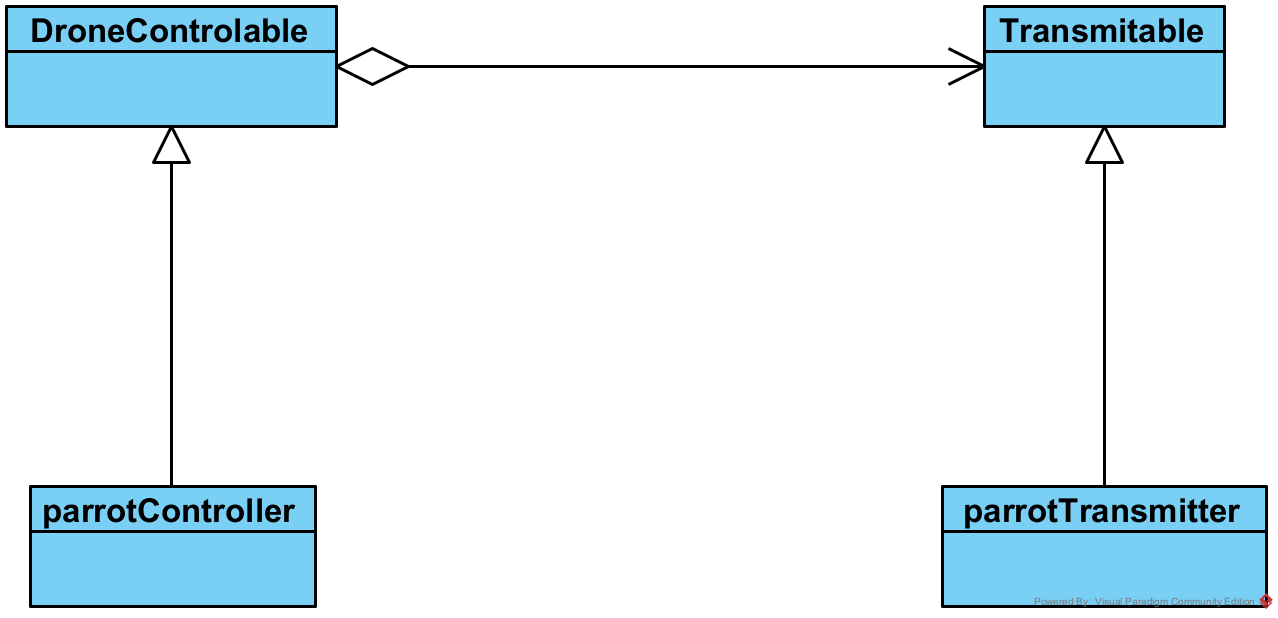
\includegraphics[width=8cm]{Pictures/Bridge.png}}
\caption{Brücke im Projekt}
\label{fig:Bridge}
\end{center}

\vspace{0.25cm}
\end{figure}


\newSec[Akteure]{Akteure\footnote{Anhand https://www.geeksforgeeks.org/bridge-design-pattern/}}{4}
\begin{tabular}{ll}
Basis-Paket:		& DroneController\\
erbendes Packet:	& parrot
\end{tabular}
\begin{table}[!ht]
\begin{tabular}{ll}
Akteur			& Klassenbezeichnung \\ \hline
Abstraction		& DroneControlable\\
RefinedAbstraction	& parrotControl\\
Implementor		& Transmitable\\
ConcreteImplementor	& parrotTransmitter\\
\end{tabular}
\end{table}


\newSec{Motivation}{4}
Das ist eine Design-Entscheidung, um im weiteren Lebenszyklus der \textit{Application} verschiedene Drohnen als \textit{PlugIn} einbinden zu können.











